% Copyright 2024 Kieran W Harvie. All rights reserved.

\section{The Blossoming of a Cubic Bézier Triangle}
We take $F=\mathbb{R}$, $N=\mathbb{R}^2$, and $M=\mathbb{R}^m$
comonly $m$ is $2$ or $3$.
\begin{center}
\begin{tikzpicture}[every node/.style={black}]
	\coordinate (e0) at (0,0);
	\coordinate (e1) at (4*0.5,4*0.86602540378);
	\coordinate (e2) at (4,0);

	\draw[-stealth] (e0)--(e1);
	\draw[-stealth] (e0)--(e2);

	\filldraw (e0) node[left]{$\mathbf{e}_0=\mathbf{0}$} circle(2pt);
	\filldraw (e1) node[above]{$\mathbf{e}_1=\mathbf{b}_1$} circle(2pt);
	\filldraw (e2) node[right]{$\mathbf{e}_2=\mathbf{b}_2$} circle(2pt);
\end{tikzpicture}
\end{center}

Cubic case
\[\mathbf{t} = \lambda_0\mathbf{e}_0+\lambda_1\mathbf{e}_1+\lambda_2\mathbf{e}_2\]
\[b(\mathbf{t}) = \lambda_0b(\mathbf{e}_0)+\lambda_1b(\mathbf{e}_1)+\lambda_2b(\mathbf{e}_2)\]
\[\begin{aligned}
	b(\mathbf{t},\mathbf{t})=& \lambda_0^2b(\mathbf{e}_0,\mathbf{e}_0)+\lambda_1^2b(\mathbf{e}_1,\mathbf{e}_1)+\lambda_2^2b(\mathbf{e}_2,\mathbf{e}_2)\\
	&+2\lambda_0\lambda_1b(\mathbf{e}_0,\mathbf{e}_1)+2\lambda_1\lambda_2b(\mathbf{e}_1,\mathbf{e}_2)+2\lambda_1\lambda_2b(\mathbf{e}_1,\mathbf{e}_2)
\end{aligned}\]

each argument can have a different $\mathbf{t}$

\begin{center}
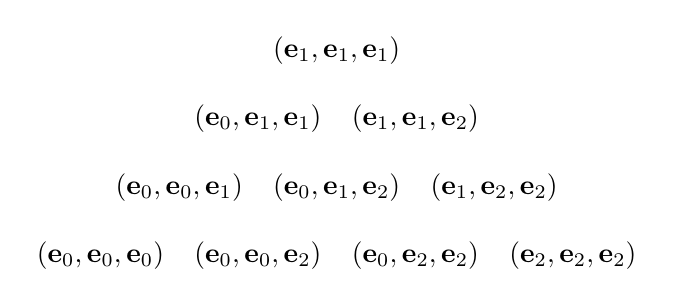
\begin{tikzpicture}[every node/.style={black}]
%	\coordinate (    ) at (Y+Z*2    , Y*1.7320508075    );
	\coordinate (e000) at (0+0*2, 0*0.86602540378);
	\coordinate (e001) at (1+0*2, 1*0.86602540378);
	\coordinate (e002) at (0+1*2, 0*0.86602540378);
	\coordinate (e011) at (2+0*2, 2*0.86602540378);
	\coordinate (e012) at (1+1*2, 1*0.86602540378);
	\coordinate (e022) at (0+2*2, 0*0.86602540378);
	\coordinate (e112) at (2+1*2, 2*0.86602540378);
	\coordinate (e122) at (1+2*2, 1*0.86602540378);
	\coordinate (e222) at (0+3*2, 0*0.86602540378);
	\coordinate (e111) at (3+0*2, 3*0.86602540378);

	\filldraw (e000) node{$(\mathbf{e}_0,\mathbf{e}_0,\mathbf{e}_0)$};
	\filldraw (e001) node{$(\mathbf{e}_0,\mathbf{e}_0,\mathbf{e}_1)$};
	\filldraw (e011) node{$(\mathbf{e}_0,\mathbf{e}_1,\mathbf{e}_1)$};
	\filldraw (e002) node{$(\mathbf{e}_0,\mathbf{e}_0,\mathbf{e}_2)$};
	\filldraw (e012) node{$(\mathbf{e}_0,\mathbf{e}_1,\mathbf{e}_2)$};
	\filldraw (e111) node{$(\mathbf{e}_1,\mathbf{e}_1,\mathbf{e}_1)$};
	\filldraw (e022) node{$(\mathbf{e}_0,\mathbf{e}_2,\mathbf{e}_2)$};
	\filldraw (e112) node{$(\mathbf{e}_1,\mathbf{e}_1,\mathbf{e}_2)$};
	\filldraw (e122) node{$(\mathbf{e}_1,\mathbf{e}_2,\mathbf{e}_2)$};
	\filldraw (e222) node{($\mathbf{e}_2,\mathbf{e}_2,\mathbf{e}_2)$};
\end{tikzpicture}\quad\begin{tikzpicture}[every node/.style={black}]
	\filldraw (e001) node{$(\mathbf{e}_0,\mathbf{e}_0,\mathbf{t})$};
	\filldraw (e011) node{$(\mathbf{e}_0,\mathbf{e}_1,\mathbf{t})$};
	\filldraw (e012) node{$(\mathbf{e}_0,\mathbf{e}_2,\mathbf{t})$};
	\filldraw (e111) node{$(\mathbf{e}_1,\mathbf{e}_1,\mathbf{t})$};
	\filldraw (e112) node{$(\mathbf{e}_1,\mathbf{e}_2,\mathbf{t})$};
	\filldraw (e122) node{$(\mathbf{e}_2,\mathbf{e}_2,\mathbf{t})$};
\end{tikzpicture}
\end{center}

\[\begin{aligned}
	b(\mathbf{t},\mathbf{t},\mathbf{t})=& \lambda_0^3b(\mathbf{e}_0,\mathbf{e}_0,\mathbf{e}_0)+\lambda_1^3b(\mathbf{e}_1,\mathbf{e}_1,\mathbf{e}_1)+\lambda_2^3b(\mathbf{e}_2,\mathbf{e}_2,\mathbf{e}_2)\\
	&+3\lambda_0^2\lambda_1b(\mathbf{e}_0,\mathbf{e}_0,\mathbf{e}_1)+3\lambda_0^2\lambda_2b(\mathbf{e}_0,\mathbf{e}_0,\mathbf{e}_2)\\
	&+3\lambda_1^2\lambda_0b(\mathbf{e}_0,\mathbf{e}_1,\mathbf{e}_1)+3\lambda_1^2\lambda_2b(\mathbf{e}_1,\mathbf{e}_1,\mathbf{e}_2)\\
	&+3\lambda_2^2\lambda_0b(\mathbf{e}_0,\mathbf{e}_2,\mathbf{e}_2)+3\lambda_2^2\lambda_1b(\mathbf{e}_1,\mathbf{e}_2,\mathbf{e}_2)\\
	&+6\lambda_0\lambda_1\lambda_2b(\mathbf{e}_0,\mathbf{e}_1,\mathbf{e}_2)\\
\end{aligned}\]
